\documentclass[12pt]{article}

\usepackage[margin=1in]{geometry}
\usepackage{amsmath}
\usepackage{booktabs}
\usepackage{enumitem}
\usepackage{hyperref}
\usepackage{graphicx}
\usepackage{icomma}
\usepackage{makecell}
\usepackage{microtype}
\usepackage{multirow}
\usepackage{tabularx}
\usepackage{textcomp}


\newcolumntype{Y}{>{\centering\arraybackslash}X}
\newcommand{\cell}[2]{\makecell[t]{$#1$ \\ $(#2)$}}

\newlength{\rowskip}
\setlength{\rowskip}{2em}

\newcommand{\oneS}{\textsuperscript{*}}
\newcommand{\twoS}{\textsuperscript{**}}
\newcommand{\threeS}{\textsuperscript{***}}

\newcommand{\age}{%
    \ifmmode\ensuremath{\text{age}}\else\textit{Age}\fi
}
\newcommand{\educ}{%
    \ifmmode\ensuremath{\textrm{education}}\else\textit{Years of education}\fi
}
\newcommand{\urban}{%
    \ifmmode\ensuremath{\textrm{urban}_i}\else\textit{Urban resident}\fi
}
\newcommand{\poorest}{\textit{In poorest two quintiles}}
\newcommand{\married}{%
    \ifmmode\ensuremath{\textrm{married}_i}\else\textit{Married}\fi
}
\newcommand{\employed}{%
    \ifmmode\ensuremath{\textrm{employed}_i}\else\textit{Employed}\fi
}
\newcommand{\catholic}{\textit{Catholic}}
\newcommand{\muslim}{\textit{Muslim}}
\newcommand{\television}{\textit{Has a television at home}}
\newcommand{\readonline}{\textit{Has read about contraception online}}

\newcommand{\outcome}{\ensuremath{\textrm{contraceptive usage}_i}}
\newcommand{\treatment}{\ensuremath{\textrm{RH Law}_i}}


\title{Estimating the effect of the Philippines' Reproductive Health Law on young women's demand for modern family planning}
\author{Eric M. Ordonez\thanks{
    This is a final research paper written for the course Program Evaluation in Developing Economies (ECON 451), taken at the University of Illinois Urbana--Champaign.
    The task was to pick a developing country and identify some exogenous shock, intervention, or something similar, then estimate the effect it had on some outcome at the micro level.
    The course also covered randomized control trials, difference-in-difference estimations, and identification assumptions and strategies.
}}
\date{}

\begin{document}
\maketitle
\begin{abstract}
    The Philippines passed the Responsible Parenthood and Reproductive Health Act of 2012 and began its implementation in 2014.
    The delayed implementation was due to the Supreme Court immediately halting it in response to challenges until they upheld its constitutionality in 2014.
    One of the law's provisions is comprehensive sex education for all public school students in Grade 5 through high school.
    
    This paper details a quasi-experiment with high-school aged girls divided into two cohorts, one each that completed high school before and after the 2014 ruling, and measures their use of or intent to use modern methods of contraception.
    A secondary analysis of the 2017 Philippines Demographic and Health Survey finds no significant effect of high school sex education in determining contraceptive usage.
    The most significant positive predictors of use are marital and employment status, with urban residency exhibiting a significantly negative effect.
\end{abstract}
\pagebreak
\tableofcontents


\pagebreak
\section{Introduction}
Demands for family planning resources and services are increasing worldwide.
The difficulties in meeting these rising demands are especially pertinent for developing countries, where high population growth can crowd out relative economic growth and stunt per capita growth.
This contributes to the well documented poverty trap where poor families continue to bear children in poverty and stay poor due to their sheer size.
The use of safe and effective methods of contraception allows families to determine the frequency and occurrence of their pregnancies and hedge against this (Gakidou \& Vayena, 2007).
But despite widespread knowledge of contraceptive methods in even the poorest countries, actual access to and use of contraceptives is lacking for myriad reasons.
In countries where public provision is limited, education is a consistent predictor of usage (Bbaale \& Mpuga 2011).

To further explore these findings, I examine the effect of high school sex education on the usage of modern contraceptives in the Philippines.
I conduct a secondary analysis of the 2017 Philippines Demographic and Health Survey (DHS).
The country's Responsible Parenthood and Reproductive Health Act of 2012 (RH Law) guarantees universal access to contraceptives, sex education, and maternal care.
I use the 2014 implementation of this law as the cutoff criterion for a quasi-experiment wherein those aged 15--16 or 18--19 in 2014 are taken as a treatment and control group, respectively.
This acts as a measure for exposure to high school sex education controlled against those who completed high school with no such exposure before the law's implementation.

Ordinary least squares regression of the usage of or intent to use a modern method of contraception on this treatment variable shows no significant effect.
I find the most significant predictors of contraceptive usage in this age range to be marital and employment status, each exhibiting an increase in likelihood; and urban residency with a negative effect, suggesting that those in rural communities are more likely to use modern methods than urban dwellers.

I explore a potential differential effect via a difference-in-difference estimate of the treatment effect across the employed and unemployed.
The treatment is again insignificant, while the differential effect is significantly positive.
Marital status and urban residency exhibit the same effects at similar magnitudes and levels of significance as in the original regression.

The initial finding is that age-related factors like marital and employment status are more powerful predictors of contraceptive usage than any effect of this treatment.
The internal validity of this finding is threatened by limitations in the data and design.
The DHS data cannot account for any variation in the quality of schools that the surveyed women attend, which is where they receive this sex education; nor does the design guarantee that the implementation was consistent for every school in the country---being provided for by law does not guarantee local compliance.
These threaten my identification assumption and the validity of what the designed treatment can actually measure.


\section{Background}
    \subsection{Family planning needs among the poor}
    Those with the greatest need and demand for family planning resources are often among the poorest socioeconomic strata.
    This is especially seen in developing countries where bearing numerous children becomes financially difficult and even dangerous to the mother, if maternal care services are lacking.

    Consequently, there is a consistent demand for contraceptive methods, but these needs are not always met due to lack of access, lack of awareness, cost, and myriad other reasons.
    As these countries grow economically, the quality and coverage of reproductive health services also grow, as well as these countries' fiscal ability to address these unmet needs.
    Making these services and resources available is a powerful determinant of actual access and usage, which is a prompt for government and international action (Gakidou \& Vayena, 2007).


    \subsection{Education and contraceptive usage}
    Evidence from developing countries suggests a key connection between education and contraceptive usage.
    Bbaale and Mpuga (2011) find that educational attainment in both men and women, particularly at the secondary and post-secondary levels, is positively associated with access to and use of contraceptives in Uganda.
    Knowledge of family planning is near universal in Uganda, but the proportion of women who have used any form of contraception, let alone a modern method, is small.
    The researchers do find lower usage rates in rural areas but attribute this to the usually lower levels of education and disproportionately smaller amounts of government spending in rural areas.
    Overall, educational attainment is a consistently positive predictor of contraceptive usage, regardless of wealth or marital status.


    \subsection{Contraception and Catholicism}
    Educational limitations can affect women's access to and use of modern contraceptives, but culture also influences attitudes that can positively or negatively affect that usage.
    The Catholic Church has historically opposed all forms of artificial birth control, and debates persist despite states secularizing
    over time and the Church's once explicit role in individual choices, like family planning, diminishing.
    These debates figure prominently in developing countries with Catholic majorities that still self-identify as more religious than secular, such as in Latin America or the Philippines.

    Hirsch (2008) surveyed a town in rural Mexico where religious (Catholic) regulations are pervasive in day-to-day affairs.
    She finds a trend, despite generational differences and social contexts, of women of all ages able to interpret and use religious reasoning to justify the use of contraceptives in their family planning decisions.
    Moreover, they can do so without jeopardizing their public standing or self-identification as devout Catholics.
    This suggests that for the cultural component of predicting contraceptive usage, being Catholic by itself may not prevent individual choices/desires to utilize contraception, provided that public access is not explicitly inhibited by a Catholic (or any other religious) institution.


    \subsection{In the Philippines}
    The Philippines is the third-largest Catholic country in the world following Brazil and Mexico.
    Evidence from Mexico (Hirsch, 2008) suggests that Catholic mores do not necessarily prevent Catholics from deciding to use contraception, which is pertinent for the Philippines.
    Compared to neighboring developing countries, the Philippines has high fertility rates and low rates of modern contraceptive usage.
    This is of great concern for the government and public health officials, as explosive economic growth is propelling the country from lower- to upper-middle income status despite roughly a fifth of the population still in poverty.

    Mello et al.\ (2006) find that a web of political, cultural, and legal barriers in the Philippines have impeded widespread access to family planning resources.
    They find that both the presence/absence of laws and their incomplete or inefficient implementation directly affect such access.
    They identify legal ambiguities, for example in what is required to access certain resources or in prescriptive authority in more remote regions, as having both positive and negative effects in provision of contraceptives.
    Thus, the Philippine government has both direct and indirect influence that it can use to promote contraceptive usage.

    However, Mello et al.\ caution that legal reform by itself will not address these issues due to opposition that has persisted long before their study: The Catholic Church and then-President Gloria Macapagal Arroyo, who typified numerous politicians' refusal to direct national funds toward public provision of modern contraceptives, due to religious reasons.
    This underlines the claim of Mello et al.\ that politics is a peripheral problem secondary to culture in the Philippines, but they also stress that effective laws shape cultural attitudes over time.
    Therefore, any legislation intended to promote use of contraceptives will also have to address the inefficiencies and cultural barriers that the review by Mello et al.\ highlights.


    \subsection{The Reproductive Health Law}
    Then-President Benigno Aquino III signed the Responsible Parenthood and Reproductive Health Act of 2012, informally known as the Reproductive Health Law and herein as the RH Law, into effect in December 2012.
    The law as written guarantees universal access to resources on contraception, fertility control, sex education, and maternal care.
    Although it officially commenced the following month, challenges from the Catholic Church and politicians across all parties ultimately brought in the Supreme Court of the Philippines.
    The Supreme Court issued an order halting implementation of all parts of the law while they heard arguments over the constitutionality of the law and its provisions.
    In April 2014, they upheld it as constitutional.

    Given how extensive Catholic influences are in Philippine politics and culture and given how inefficient preexisting laws and institutions have been, the RH Law represents a landmark attempt by the government in promoting family planning.
    The demand for family planning in developing countries is well understood, and positive associations between education and contraceptive access/usage are well documented.
    Therefore, the effect of sex education on contraceptive usage is a suitable topic for evaluation and will be the focus of this paper.


\section{Data}
    \subsection{Philippines Demographic and Health Survey}
    This paper is a secondary analysis of the 2017 Philippines Demographic and Health Survey (DHS), with fieldwork conducted by the Philippine Statistics Authority (PSA) from August to October 2017.
    Data were collected from interviews at the household and individual levels, representing 25,074 women aged 15--49 occupying 27,496 households across all 17 administrative regions.
    Therefore, it can be considered a representative sample of Filipina women of reproductive age nationwide who could be in need of modern
    contraceptives.

    The household and individual data sets are merged so as to match household characteristics to individual respondents.
    Specifically, the sample under study is the subset of women who were aged 15--16 or 18--19 in 2014, corresponding to being aged 18--19 and 21--22 at the time of their interviews.
    There are 3,473 such observations, which is the largest number that satisfies these identification criteria and for which there are non-missing records for all relevant variables.
    (Only 10 observations with missing records were dropped from an original 3,483).


    \subsection{Variable choice and definitions}
    I measure the outcome of this intervention by usage of or intent to use modern methods of contraception, per
    DHS definitions.\footnote{
        According to the DHS, modern methods include male and female sterilization, injectables, intrauterine devices (IUDs), contraceptive pills, implants, the patch, female and male condoms, emergency contraception, the standard days method (SDM), mucus/Billings/ovulation, basal body temperature, symptothermal, and the lactational amenorrhea method (LAM).
    }
    This is generated as an indicator for whether respondents were currently using a modern method or for if they intended to use one otherwise.
    With this, I estimate the effect of high school sex education following implementation of the RH Law via its impact on the likelihood of using modern methods.

    I identify ten potential control variables to examine baseline balances between the treatment and control groups, each for reasons that I anticipate may also have explanatory effects on the outcome thanks to the existing literature. 
    They are as follows, with their names as they appear in Tables \ref{table:summary}--\ref{table:did}:


    \begin{enumerate}
        \item \age{}
        
        How old the respondent was in years at the time of the interview.
        Naturally, one becomes more sexually aware, active, and proactive as one gets older.
        I anticipate a nonlinear relationship with the outcome due to sexual activity, on average, increasing then plateauing and decreasing past a certain age, and I control for this in the regression (see Section \ref{econometric-specification}).

        \item \educ{}
        
        How many years of education at any level the respondent had completed at the time of the interview, irrespective of whether they were still in school.
        I anticipate that more education makes one more likely to use modern methods due to a more formalized understanding of what contraception is, its uses, and how to acquire it.
    
        \item \urban{}
        
        Indicator for whether the respondent lived in an urban area, with urban-rural classifications made by the PSA at the \textit{barangay} (neighborhood) level per Census of Population and Housing data.
        Urban areas are often wealthier and better connected than rural areas, facilitating access to family planning resources.
    
        \item \poorest{}
        
        Indicator for if the respondent belonged to the bottom two quintiles of a wealth index.
        The DHS classifies households (poorest, poorer, middle, richer, richest) by an aggregated wealth index for observable socioeconomic indicators such as water supply, sanitation, electricity, and materials used for housing construction.
        Those in higher socioeconomic strata should be more aware of and able to access family planning resources.
    
        \item \married{}
        
        Indicator for marital status.
        Married couples are more likely to want children and engage in sexual activity with only each other, suggesting a decreased need for contraception.

        \item \employed{}

        Indicator for if the respondent was currently working at the time of the interview.
        The pressures of hard labor or of a full-time career may convince one to delay having children, prompting a demand for family planning.
        This variable is generated according to if the respondent was working with any regularity at the time of the interview, regardless of the nature of the work.
    
        \item \catholic{}
        
        Indicator for if the respondent professed to be Catholic.
        The Philippines is overwhelmingly Christian, with 80.58\% of the population belonging to the Catholic Church and 11.66\% to other
        denominations.\footnote{
            Per the most recent available data dated 2010, reported by the 2015 PSA Census of Population.
        }
        The most vocal opposition to the RH Law and to sex education in schools comes from the Catholic Church, and Catholic influences are ingrained in Filipino culture and society due to three centuries of Spanish colonial rule.
    
        \item \muslim{}
        
        Indicator for if the respondent professed to be Muslim. 
        Islam is the second largest religion by adherents at 5.57\% of the population,\footnote{
            \textit{Ibid.}    
        }
        with a significant presence in the south predating
        the arrival of the Spanish and Christianity (a region that is largely poorer than the rest of the country too).
        I anticipate a religious effect in the same vein as the
        Catholic Church's opposition.

        \item \television{}

        Indicator for if the respondent had a television in their home. 
        The DHS finds that television is the most popular form of mass media among women in the Philippines and is the primary medium through which they hear about family planning, as 77\% of women watch it at least once a week.
    
        \item \readonline{}

        Indicator for if the respondent had read about contraception on
        the Internet in the past 12 months.
        The Internet is the second most popular form of mass media among
        women, with 68\% using it in the past 12 months.
    \end{enumerate}

    Sample summary statistics for these variables are given in Table \ref{table:summary}, Column 1.
    The average age of the sample is 19.877 with an average 11.381 years of completed formal education.
    The proportion of respondents living in urban areas is 38.1\%, with 44.1\% of respondents being in the poorest two quintiles.
    Average marriage and employment rates are 10.4\% and 37.3\%, respectively; 71.8\% of the sample are Catholic, while 10.8\% are Muslim; 75.2\% have a television at home, and 45.3\% had read about contraception online within the previous year.


\section{Empirical approach}
    \subsection{Identification strategy}
    Although the RH Law was officially enacted in December 2012 and commenced in January 2013 as expected, no timetable could be put on its full implementation.
    The Supreme Court challenged its constitutionality in March and blocked implementation of its provisions for four months, with the status quo then extending into the next year while they deliberated official petitions opposing the law.
    It was uncertain whether the law would be upheld, struck down, or sent for amendment.
    Schools, students, administrators, and local government units could not prepare for curriculum or lifestyle changes that were unsure would come.
    So when the Supreme Court ruled in April 2014 that the RH Law is constitutional, allowing for its immediate implementation (albeit with eight provisions struck down, none related to sex education), the entire country experienced an exogenous shock in health and education policy.

    I conduct a quasi-experiment based on this ruling.
    Since the academic year typically ends in April, I assume that sex education pursuant to the RH Law would take effect for subsequent school years.
    Thus, anyone aged 15--16 at that time would have at least two years of high school completed without sex education implemented due to the RH Law and at least one more year left with it.
    On the other hand, anyone aged 18--19 at that time would have graduated and thus have a complete high school education identical to the so-far completed part of the younger cohort's education.
    The former thereby constitutes a treatment group, the latter a control group.

    I exploit this differentiation to estimate this treatment effect via a regression analysis of observable outcomes.
    This requires an identification assumption that these two groups are identical across observable and unobservable characteristics.
    This would imply that any variation in modern contraceptive usage can be attributed only to this difference in high school sex education.
    I compare averages of the ten aforementioned variables, which I also choose as representative population characteristics, across the two groups to verify this assumption; an assumed balance for each characteristic implies that the group differences for each one should not be statistically significantly different from zero.

    Table \ref{table:summary}, Columns 2--4 show this balancing.
    The average age of the treatment group is 18.482; the control group, 21.518.
    The difference (\textminus3.036) is statistically significant at the 1\% level but is of course by construction, as I choose a three-year gap in ages to differentiate the two groups about 2014.
    Nevertheless, with the hypothesized positive relationship between age and contraceptive usage over the sample’'s age range, this difference can bias the estimated effect on the treatment group downward.
    \age{} is thus included as a control variable in the regression.

    The two groups also differ significantly in years of education, marital status, and employment status at the 1\% level.
    Overall on average, those in the control completed 11.755 years of formal education, 17.4\% of them are married, and 50.3\% are employed; whereas those in the treatment are less likely to be married (4.5\%) and employed (26.2\%) by 12.8 and 24.1 percentage points (pp), respectively, and they had completed on average 0.693 fewer years of education (11.063).

    These imbalances may correlate with the age imbalance.
    Given the contemporary age ranges (treatment: 18--19, control: 21--22), those in the control are reasonably more likely to have completed more post-secondary education, to be in the workforce, and to be married than those in the treatment, many of whom are just recently graduated from high school.
    Since the age imbalance is introduced by design, \educ{}, \married{}, and \employed{} are also included as control variables in the analysis.
    This is to mitigate potential downward (\educ{}, \employed{}) and upward (\married{}) biases on the treatment effect, as the former two variables have a hypothesized positive effect on the outcome, the latter a negative effect.

    The difference in urban residency is significant at the 10\% level; 39.8\% of the control group live in urban areas, but those in the treatment group are 3.2 pp less likely to (36.7\%).
    This difference is not as plausibly attributable to the constructed age difference, so the two groups are not identical in this regard. Hence, \urban{} is included as the last control variable to account for any potential downward bias due to its hypothesized
    positive relationship with the outcome.

    Since group mean differences for the remaining variables (\poorest{}: \textminus0.009, \catholic{}: \textminus0.001, \muslim{}: 0.000, \television{}: 0.019, \readonline{}: 0.023) are all statistically insignificant, the groups are assumed to be identical in these regards, thereby omitting them as controls.


    \subsection{Econometric specification} \label{econometric-specification}
    The anticipated causal relationship is expressed by the simple regression
    \begin{equation}
        \label{eq:1}
        \outcome = \alpha + \beta \: \treatment + \varepsilon,
    \end{equation}
    where ``contraceptive usage,'' as an indicator, is the likelihood of using or intending to use modern methods of contraception, and ``RH Law'' is the treatment of receiving sex education in high school as mandated by the RH Law.
    The coefficient $\beta$ therefore represents how much more likely one is to use a modern method given a high school sex education pursuant to the RH Law than one who did not receive such an education.

    Equation \ref{eq:1} represents a naive model that does not account for biasing effects from population imbalances.
    Thus, the previously specified control variables are introduced to explain this variation and express the causal relationship as the multiple regression
    \begin{align}
    \begin{split}
        \label{eq:2}
            \outcome &= \alpha + \beta_1 \: \treatment + \beta_2 \: \age + \beta_3 \: \age^2 + \beta_4 \: \educ \\
            &\qquad + \beta_5 \, \urban + \beta_6 \: \married + \beta_7 \: \employed + \varepsilon.
    \end{split}
    \end{align}

    Among the new variables, ``$\age$'' and ``$\age^2$'' for \age{} and $\educ$ for \educ{} are quantitative measures; the rest are qualitative.
    Each $\beta_i$ represents the individual impact each variable has on the likelihood of modern contraceptive usage except for $\beta_2$ and $\beta_3$, since \age{} exhibits a nonlinear relationship with this outcome (see Figure \ref{fig:1}).
    Those two terms must be considered in tandem.

    Each coefficient's anticipated sign corresponds to its hypothesized relationship with contraceptive usage.
    The data suggest that contraceptive usage increases, plateaus, then decreases with age, so $\beta_2$ should be positive and $\beta_3$ negative to approximate this quadratic trend.
    Education, urban residency, and employment are hypothesized to have a positive effect, so the corresponding coefficients $\beta_4$, $\beta_5$, and $\beta_7$ should be positive.
    Marital status is hypothesized to have a negative effect, so $\beta_6$ should be negative.
    Sex education (the treatment) should have a positive effect, so $\beta_1$ should be positive.

    Significance in the regression estimate of Equation \ref{eq:2} (see Table \ref{table:regression}, Column 6) motivates investigating potential differential effects among the control variables.
    I choose employment status due to its statistically significant positive effect on contraceptive usage, as was anticipated. 
    Introducing an interaction term between it and the treatment gives a difference-in-difference specification
    \begin{equation}
        \label{eq:3}
        \outcome = \alpha + \beta_1 \: \treatment + \beta_2 \: \treatment \cdot \employed + \beta_3 \: \employed + \varepsilon,
    \end{equation}
    where the coefficient $\beta_2$ is the differential effect of the treatment across those who are employed and those who are unemployed. 
    Due to the hypothesized individual positive relationships of each variable, the difference-in-difference is hypothesized to be positive too.

    The remaining control variables are introduced into Equation \ref{eq:3} to mitigate biases due to imbalances, giving the full model as
    \begin{align}
    \begin{split}
        \label{eq:4}
        \outcome &= \alpha + \beta_1 \: \treatment + \beta_2 \: \treatment \cdot \employed \\
        &\qquad + \beta_3 \: \age + \beta_4 \: \age^2 + \beta_5 \: \educ \\
        &\qquad + \beta_6 \: \urban + \beta_7 \: \married + \beta_8 \: \employed + \varepsilon.
    \end{split}
    \end{align}


\section{Results}
The main treatment effect under study is how exposure to high school sex education following the 2014 implementation of the RH Law has impacted young women's inclination to use modern methods of contraception.


    \subsection{Regression estimates}
    An estimate of the naive model, a simple regression of contraceptive usage on sex education (Equation \ref{eq:1}), is given in Table \ref{table:regression}, Column 1.
    The likelihood of using modern contraceptives among those without RH Law sex education is given by the constant term: 0.566.
    Yet the coefficient of the treatment term suggests that that education decreases this likelihood by 6.2 pp, a finding contrary to what was expected.
    This seemingly has explanatory power due to both terms being significant at the 1\% level.

    Compare this to the results of the full regression (Equation \ref{eq:2}) in Table \ref{table:regression}, Column 6.
    In addition to the treatment, the full regression includes the control variables that have statistically significant differences across the treatment and control groups.
    Living in an urban area, being married, and being employed are all significant at the 1\% level.
    Urban dwellers are 4.1 pp less likely to use modern methods than rural dwellers, not more likely as anticipated.
    Married women are 13.2 pp more likely to use modern methods than unmarried women, not less likely as anticipated.
    The employed are 6.7 pp more likely than the unemployed to use modern methods, as anticipated.
    The effects of age and education are both statistically insignificant; additional years of schooling have virtually no effect, while the linear and quadratic components of age agree with what was hypothesized and with what is seen in Figure \ref{fig:1}.

    Notably, the treatment goes from being statistically significant ($\beta_1 = -0.062$) at the 1\% level to insignificant ($\beta_1 = 0.019$).
    This confirms that the treatment in the naive model captures variation from other factors, thus biasing this estimate of its effect.

    Assignment to the treatment group was random in that respondents had no control over when they were born, as the inclusion criterion was an age cutoff.
    But the treatment and control groups are necessarily different in age by construction.
    It is possible that predictors of a demand for modern contraceptives that come naturally with age, such as getting married and having a job, are more powerful than the treatment measured here.
    This is seen in the significance of these effects, indicated by marital and employment status, dominating all other terms in the regression.


    \subsection{Differential effects}
    Equation \ref{eq:3} expresses the differential effect of being employed across the treatment and control groups on the outcome, which is estimated by the regression output in Table \ref{table:did}, Column 1.
    Employment status, which in Equation \ref{eq:2} was shown to be statistically significant at the 1\% level, is now insignificant, while the treatment and interaction term are both significant at the 1\% level.
    The treatment, as in the naive model, exhibits a negative effect: The unemployed who received high school sex education are 8.6 pp less likely to use modern contraceptives than the unemployed who received no such education.
    The coefficient of the interaction term indicates that the differential effect of being employed across the two groups is a 10.1 pp increase in the likelihood of using modern contraceptives.
    Notably, the constant term, significant at the 1\% level, suggests that only 5.62\% of the unemployed who did not receive high school sex education use or will use modern methods of contraception.

    Introducing the controls to this difference-in-difference specification (Equation \ref{eq:4}) yields effects consistent with those from the previous two regressions, as seen in Table \ref{table:did}, Column 2.
    The difference-in-difference between employment and the treatment, a 7.7 pp increase in the outcome, is now significant at the 5\% level.
    The treatment is again no longer significant, while marital status and urban residency are again significant at the 5\% and 1\% levels with a 12.6 pp increase and 4.0 pp decrease in the outcome, respectively.

    Both these regressions further reinforce the possibility that these age-related predictors are presently more powerful than what is measured by the treatment.
    This is seen in the significance both (1) of the difference-in-difference in employment status across the treatment and control groups and (2) of marital status, as before.


\section{Experimental limitations}
    \subsection{External validity}
    This analysis is limited in its applicability to other developing countries like the Philippines or even to other Catholic countries.
    The Philippines is unique in Asia as one of only two predominantly Catholic countries (together with East Timor), but it is the third-largest Catholic country in the world.
    Its situation with implementation of the RH Law clashing with the Catholic Church, which has tremendous political clout, cannot be immediately to any of its non-Christian neighbors despite similar levels of economic development.

    Being Catholic (or Muslim) was found to have insignificant effects in this analysis, but further exploration of these qualifiers could verify some external validity.
    For example, a measure of to what extent one's faith informs decisions about family planning and sexual activity is a potential operationalization of the Catholic sociocultural influences that are nominally at odds with the RH Law.
    Doing so could help generalize the resultant findings (even if different) to countries like neighboring Malaysia and Indonesia with overwhelming Muslim majorities, or to other Catholic countries at different levels of development but experiencing similar changes in health and education policy.

    Finally, the single measure of contraceptive usage with regards to education does limit external validity to contraceptive usage in other contexts. 
    This experiment's outcome may not necessarily be generalizable since a need for family planning can go unmet (which is recorded as ``not using'' in this design) due to a variety of confounding financial, educational, and cultural factors.
    Education may have a true positive effect that could be repeatedly seen in other countries but that is suppressed here due to financial and cultural circumstances unique to the Philippines, for example.


    \subsection{Internal validity}
    A threat to this study's internal validity is omitted variable bias. 
    The DHS collects data on women only at the individual and household levels; thus, there is unaccounted and likely significant variation in the quality of schools that the surveyed women attend.
    This threatens the identification assumption due to potential imbalances both between and within the experimental groups along dimensions relevant to the treatment effect.
    A causal effect of receiving sex education on contraceptive usage could vary with the kind of educational materials available, the frequency and breadth of lessons, and the possibility of spreading misinformation.
    The treatment could be better operationalized with proper measures and indicators for the sex education actually delivered to these women.

    The current operationalization does not guarantee complete treatment either.
    An indicator for ``being exposed to sex education'' may be ambiguous or even falsely positive if schools, administrators, and local government units do not comply with the law's requirements.
    However, any kind of compliance is questionable if the Departments of Education and Health cannot agree upon what sex education in schools should entail, which is not accounted for in the data nor this study.
    Although the Department of Education includes comprehensive sex education in the official K--12 curriculum, minimum standards for it that can be enforced nationwide have yet to be developed (as of December 2018).
    One consequence of this is that teachers are not trained how to best deliver age-specific content, so there is therefore no way to ensure a theoretically consistent education even at the high school level. 
    Again, this variation in school environments threatens the identification assumption and the validity of what the designed treatment can actually measure.


\section{Conclusion}
This paper presents a secondary analysis of the 2017 Philippines DHS to estimate the effect of high school sex education, following the 2014 implementation of the RH Law, on the use of or intention to use modern methods of contraception.
I find no significant relationship between the treatment and usage of modern contraceptives, with the most significant predictors of contraceptive use being marital status, employment status, and urban residency.
Married women are 13.2 pp more likely to use modern methods than unmarried women, employed women are 6.7 pp more likely than unemployed women, and women living in urban areas are 4.1 pp less likely than women in rural areas.
I also find a significant differential effect of employment status across the treatment and control groups.
The difference-in-difference is a 7.7 pp increase, with urban residency and marital status exhibiting similar effects as in the main regression: A 4.0 pp decrease and 12.6 pp increase, respectively.

These results suggest that sex education by itself has no significant effect on women's decision or intent to use modern methods of contraception.
Instead, the effects of age-related factors, such as joining the workforce or getting married, dominate.
Contraceptive usage exhibits a nonlinear relationship with age but with a positive trend over the age range in this study.
Thus, the results reflect this natural increase over time, as older women are more likely to be married and employed.
The negative effect of urban residency is consistent with past observations that rural regions, which are typically poorer, have a greater demand for family planning to reduce fertility where it is difficult or dangerous to continue bearing children.

The differential effect of employment status has no immediately obvious interpretation.
Due to the age discrepancy between the treatment and control groups, an employed woman who received sex education would be aged 18--19 compared to an employed woman who did not and who would be aged 21--22.
The former is perhaps someone who forewent higher education to work straight away, while the latter may have gone to college before working.
An older and potentially college-educated woman may be readier to start a family and in a better position to do so, hence a lower demand for contraceptives to delay childbirth compared to, say, a teenager who is working but not yet ready to support any children she could potentially bear.
One way to investigate this would be to determine the differential effect of marital status across the treatment as well as the double differential effect of employment and marital statuses by looking at the difference-in-difference-in-differences between the married, the employed, and the treated.

Overall, the data suggest that it is too soon to evaluate the efficacy of sex education under the RH Law at this scale.
Although there are significant effects worth exploring, there is not enough information available so as to control for variation in school quality and further isolate the desired effect of sex education.
A more robust treatment could be a randomized control trial of the use of certain sex education materials in schools with similar resources across regions of similar economic and urban development, but this is prohibitively difficult with the data available in the DHS alone.
The actual implementation of the RH Law also poses a problem, as not all its provisions have been consistently deployed in all parts of the country despite its status as law for four years now.
In this case, meaningful nationwide evaluation of sex education may not be possible until the Department of Education can guarantee minimum standards for comprehensive sex education and that schools can meet them.


\section{References}
% \raggedright
\begin{enumerate}[label={[\arabic*]}]
    \item Bbaale, E. \& Mpuga, P. (2011). Female Education, Contraceptive Use, and Fertility: Evidence from Uganda. \textit{Consilience: The Journal of Sustainable Development,} \textit{6}(1), 20--47.
    \item Gakidou, E. \& Vayene, E. (2007). Use of Modern Contraception by the Poor Is Falling Behind. \textit{PLoS Medicine,} \textit{4}(2). \url{https://doi.org/10.1371/journal.pmed.0040031}.
    \item Hirsch, J.S. (2008). Catholics Using Contraceptives: Religion, Family Planning, and Interpretive Agency in Rural Mexico. \textit{Studies in Family Planning,} \textit{39}(2), 93--104.
    \item Mello, M.M., Powlowski, M., Nañagas, J.M.P., and Bossert, T. (2006). The role of law in public health: The case of family planning in the Philippines. \textit{Social Science \& Medicine,} \textit{63}, 384--396.
    \item Philippine Statistics Authority (PSA) and ICF. (2018). Philippines National Demographic and Health Survey 2017. Quezon City, Philippines, and Rockville, Maryland, USA: PSA and ICF.
    \item Philippine Statistics Authority. (2015). 2015 Census of Population. Quezon City, Philippines: PSA. Available from \url{https://psa.gov.ph/tags/popcen-2015}.
\end{enumerate}


\pagebreak
\section{Appendix}
% Figure 1
\begin{figure}[ht]
    \centering
    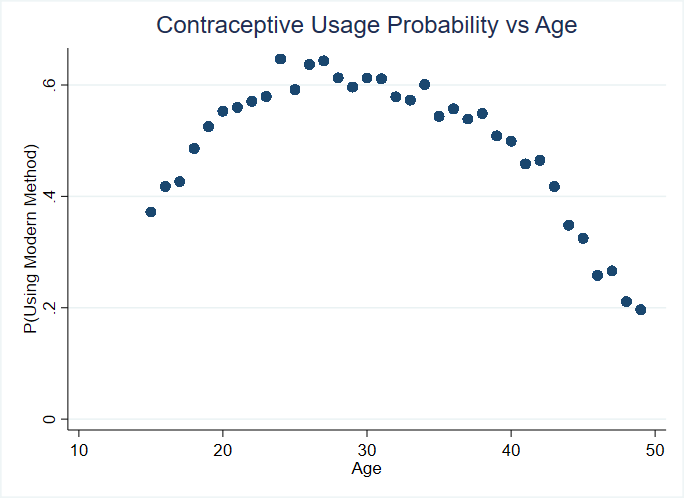
\includegraphics[width=\textwidth]{figures/fig1.png}
    \caption{
        \label{fig:1}
        Evidence of the nonlinear relationship between age and contraceptive usage.
        Probability of using modern methods of contraception is the mean of the outcome indicator for every age in years in the data, 15--49.
        An age squared term is added to the analysis instead of a cubic or B-spline interpolant since the nonlinear component is desired only over the age range in the sample, 18--22 (before the bend).
        Age squared was deemed sufficient for this.
    }
\end{figure}

% Table 1
\begin{table}[ht]
    \centering
    \begin{tabularx}{\textwidth}{>{\raggedright}X *{4}{Y}}
        \multicolumn{5}{c}{
            \textbf{Summary statistics of sample and treatment/control groups}
            } \\
        \toprule
        & Sample & Treatment & Control & Difference \\
        & (1) & (2) & (3) & (4) \\
        \cmidrule(lr){2-5}
        Age                                 & \cell{19.877}{1.594}
                                            & \cell{18.482}{0.500}
                                            & \cell{21.518}{0.500}
                                            & $-3.036$\threeS \\[\rowskip]
        Years of education                  & \cell{11.381}{2.832}
                                            & \cell{11.063}{2.466}
                                            & \cell{11.755}{3.169}
                                            & $-0.693$\threeS \\[\rowskip]
        Urban resident                      & \cell{0.381}{0.486}
                                            & \cell{0.367}{0.482}
                                            & \cell{0.398}{0.490}
                                            & $-0.032$\oneS \\[\rowskip]
        In poorest two quintiles            & \cell{0.441}{0.497}
                                            & \cell{0.437}{0.496}
                                            & \cell{0.446}{0.497}
                                            & $-0.009$ \\[\rowskip]
        Married                             & \cell{0.104}{0.306}
                                            & \cell{0.045}{0.208}
                                            & \cell{0.174}{0.379}
                                            & $-0.128$\threeS \\[\rowskip]
        Employed                            & \cell{0.373}{0.484}
                                            & \cell{0.262}{0.440}
                                            & \cell{0.503}{0.500}
                                            & $-0.241$\threeS \\[\rowskip]
        Catholic                            & \cell{0.718}{0.450}
                                            & \cell{0.717}{0.450}
                                            & \cell{0.718}{0.450}
                                            & $-0.001$ \\[\rowskip]
        Muslim                              & \cell{0.108}{0.311}
                                            & \cell{0.108}{0.311}
                                            & \cell{0.108}{0.311}
                                            & $0.000$ \\[\rowskip]
        Has a television at home            & \cell{0.752}{0.432}
                                            & \cell{0.761}{0.427}
                                            & \cell{0.742}{0.437}
                                            & $0.019$ \\[\rowskip]
        Has read about contraception online & \cell{0.453}{0.498}
                                            & \cell{0.463}{0.499}
                                            & \cell{0.440}{0.497}
                                            & $0.023$ \\[\rowskip]
        \cmidrule(lr){2-5}
        $n$                                 & $3,473$
                                            & $1,878$
                                            & $1,595$
                                            & \\
        \bottomrule
    \end{tabularx}
    \caption{
        \label{table:summary}
        The sample is defined as the subset of women surveyed in the 2017 Philippines DHS who were aged 15--16 or 18--19 in 2014 with non-missing records for the listed characteristics, giving a total of $n = 3,473$ observations.
        The former constitutes the treatment group (Column 2), the latter the control group (Column 3).
        Sample and group means are given across Columns 1--3 with standard deviations in parentheses.
        The difference between treatment and control means is given in Column 4 with statistical significance indicated at $\oneS = 10\%$, $\twoS = 5\%$, and $\threeS = 1\%$.
    }
\end{table}

% Table 2
\begin{table}[ht]
    \centering
    \begin{tabularx}{\textwidth}{>{\raggedright}X *{6}{Y}}
        \multicolumn{7}{c}{
            \textbf{Regression estimate of effects of sex education on contraceptive usage}
        } \\
        \toprule
        & \multicolumn{6}{c}{Using or intends to use a modern contraceptive method} \\
        & (1) & (2) & (3) & (4) & (5) & (6) \\
        \cmidrule(lr){2-7}
        Sex education               & \cell{-0.062\threeS}{0.017}
                                    & \cell{0.018}{0.054}
                                    & \cell{0.019}{0.054}
                                    & \cell{0.020}{0.054}
                                    & \cell{0.018}{0.054}
                                    & \cell{0.019}{0.054} \\[\rowskip]
        Age                         &
                                    & \cell{0.218}{0.226}
                                    & \cell{0.240}{0.226}
                                    & \cell{0.235}{0.226}
                                    & \cell{0.230}{0.225}
                                    & \cell{0.204}{0.225} \\[\rowskip]
        Age\textsuperscript{2}      & 
                                    & \cell{-0.005}{0.006}
                                    & \cell{-0.005}{0.006}
                                    & \cell{-0.005}{0.006}
                                    & \cell{-0.005}{0.006}
                                    & \cell{-0.005}{0.006} \\[\rowskip]
        Years of education          &
                                    &
                                    & \cell{-0.004}{0.003}
                                    & \cell{-0.003}{0.003}
                                    & \cell{0.001}{0.003}
                                    & \cell{0.000}{0.018} \\[\rowskip]
        Urban resident              &
                                    &
                                    &
                                    & \cell{-0.046\threeS}{0.018}
                                    & \cell{-0.039\twoS}{0.018}
                                    & \cell{-0.041\threeS}{0.018} \\[\rowskip]
        Married                     &
                                    &
                                    &
                                    &
                                    & \cell{0.121\threeS}{0.030}
                                    & \cell{0.132\threeS}{0.030} \\[\rowskip]
        Employed                    &
                                    &
                                    &
                                    &
                                    &
                                    & \cell{0.067\threeS}{0.018} \\[\rowskip]
        Constant                    & \cell{0.566\threeS}{0.012}
                                    & \cell{-1.908}{2.248}
                                    & \cell{-2.088}{2.252}
                                    & \cell{-2.042}{2.250}
                                    & \cell{-1.986}{2.245}
                                    & \cell{-1.692}{2.243} \\[\rowskip]
        \cmidrule(lr){2-7}
        $R^2$                       & $0.004$
                                    & $0.005$
                                    & $0.005$
                                    & $0.007$
                                    & $0.012$
                                    & $0.016$ \\[0.5em]
        $n$                         & $3,473$
                                    & $3,473$
                                    & $3,473$
                                    & $3,473$
                                    & $3,473$
                                    & $3,473$ \\
        \bottomrule
    \end{tabularx}
    \caption{
        \label{table:regression}
        The dependent variable is defined by an indicator for whether the respondent was using or intended to use a modern method of contraception.
        This is then regressed on the treatment (Column 1) and again with sequential addition of control variables (Column 2--6).
        Control variables are those with statistically significant imbalances across the treatment and control groups as seen from Table \ref{table:summary}, Column 4, with \age{}\textsuperscript{2} added to account for the nonlinear relationship that age exhibits with the outcome (see Figure \ref{fig:1}).
        \age{}, \age{}\textsuperscript{2}, and \educ{} are quantitative variables; the rest are indicators. 
        Standard errors in parentheses.
        Statistical significance indicated at $\oneS = 10\%$, $\twoS = 5\%$, and $\threeS = 1\%$.        
    }
\end{table}

% Table 3
\begin{table}[ht]
    \centering
    \begin{tabularx}{\textwidth}{>{\raggedright}X *{2}{Y}}
        \multicolumn{3}{c}{
            \textbf{Differential effect of employment status on contraceptive usage}
        } \\
        \toprule
        & \multicolumn{2}{c}{Using or intends to use a modern contraceptive method} \\
        & (1) & (2) \\
        \cmidrule(lr){2-3}
        Sex education                               & \cell{-0.086\threeS}{0.022}
                                                    & \cell{-0.014}{0.056} \\[\rowskip]
        Sex education $\times$ Employed             & \cell{0.101\threeS}{0.036}
                                                    & \cell{0.077\twoS}{0.036} \\[\rowskip]
        Employed                                    & \cell{0.008}{0.025}
                                                    & \cell{0.029}{0.025} \\[\rowskip]
        Age                                         & & \cell{0.160}{0.226} \\[\rowskip]
        Age\textsuperscript{2}                      & & \cell{-0.004}{0.006} \\[\rowskip]
        Years of education                          & & \cell{0.001}{0.003} \\[\rowskip]
        Urban resident                              & & \cell{-0.040\twoS}{0.018} \\[\rowskip]
        Married                                     & & \cell{0.126\threeS}{0.030} \\[\rowskip]
        Constant                                    & \cell{0.056\threeS}{0.018}
                                                    & \cell{-1.225}{2.252} \\[\rowskip]
        \cmidrule(lr){2-3}
        $R^2$                                       & $0.009$ & $0.018$ \\[0.5em]
        $n$                                         & $3,473$ & $3,473$ \\
        \bottomrule
    \end{tabularx}
    \caption{
        \label{table:did}
        \textit{Sex education $\times$ Employed} is an interaction term.
        Columns 1 and 2 correspond to coefficient estimates from regressions run without and with control variables, respectively.
        Standard errors in parentheses.
        Statistical significance indicated at $\oneS = 10\%$, $\twoS = 5\%$, and $\threeS = 1\%$.
    }
\end{table}
\end{document}